\chapter{Introducción específica} % Main chapter title

\label{Chapter2}

%----------------------------------------------------------------------------------------
%	SECTION 1
%----------------------------------------------------------------------------------------

En el presente capítulo se describen las principales tecnologías utilizadas para la realización del trabajo, entre las que se incluyen herramientas de software y componentes de hardware.

\section{Protocolos de comunicación}

En esta sección se describen los protocolos de comunicación utilizados en IoT y aplicados a nuestro trabajo.


\subsection{Tecnología de comunicación Wi-Fi}
Wi-Fi es una tecnología de red inalámbrica a través de la cual diferentes artefactos como computadoras (portátiles y de escritorio), dispositivos móviles y otros equipos (impresoras, cámaras, asistentes de voz) pueden intercambiar información entre sí y con Internet \citep{WEBSITE:WifiCisco}. La principal ventaja del uso de estas tecnologías es que ahorran el cableado en los hogares o empresas, que son costosos y engorrosos de instalar. Además, permiten la movilidad de los usuarios en el área de cobertura. 

Cabe aclarar que Wi-Fi no es un acrónimo, sino una marca comercial específica propiedad de la Wi-Fi Alliance, un grupo dedicado a certificar que los productos de Wi-Fi cumplen con el conjunto de estándares inalámbricos 802.11 de la IEEE. Esta alianza garantiza que la compatibilidad entre dispositivos con la marca Wi-Fi es total, asegurando la interoperabilidad de los mismos \citep{WEBSITE:WifiEstandar}. El estándar 802.11 surgió en la década de 1990 y continúa creciendo en la actualidad. El mismo agrupa diferentes versiones de la norma,  cada una de las cuales se determinan por el rendimiento y el alcance inalámbrico, así como por la disponibilidad de nuevas frecuencias, nuevos protocolos de seguridad y tecnologías que reducen el consumo de energía.

En la tabla \ref{tab:protolocos80211} se presenta un resumen de los diferentes estándares de la norma 802.11 y sus principales características \citep{WEBSITE:80211}.

\begin{table}[h]
	\centering
	\caption[Protocolos 802.11]{Estándares de la norma 802.11 y sus principales características.}
	\begin{tabular}{p{2.5cm} p{3.5cm} p{3.5cm} p{3.5cm} } 	

		\toprule
		\textbf{Estándar} & 
		\textbf{Velocidad máxima} &
		\textbf{Frecuencia} &
		\textbf{Compatibilidad con modelos anteriores} 
		\\
		\midrule
802.11a & 4 Mbps & 5 GHz & No \\
802.11b & 11 Mbps & 2,4 GHz & No \\
802.11g & 54 Mbps & 2,4 GHz & 802.11b \\
802.11n & 600 Mbps & 2,4 GHz o 5 GHz & 802.11a/b/g \\
802.11ac & 3,46 Gbps & 5 GHz & 802.11a/n \\
802.11ad & 6,7 Gbps & 2,4 GHz, 5 GHz y 60 GHz & 802.11a/b/g/n/ac \\
802.11ah & 347 Mbps & 0,9 GHz & No \\
		\bottomrule
		\hline
	\end{tabular}
	\label{tab:protolocos80211}
\end{table}

\pagebreak
\subsection{Protocolo HTTP}

HTTP (Hypertext Transfer Protocol) es un protocolo que nos permite realizar peticiones de datos y recursos a través de Internet. Fue desarrollado por el World Wide Web Consortium (W3C) y la Internet Engineering Task Force (IETF), mediante una colaboración que culminó en 1999 con la publicación de una serie de RFCs (Request for Comments), siendo el más importante de ellos el RFC 2616 \citep{rfc2616} que especifica la versión 1.1 de éste. HTTP define la sintaxis y la semántica que utilizan los elementos de software de la arquitectura de Internet (clientes, servidores, \textit{proxies}) para comunicarse entre sí. Es un protocolo sin estado, es decir, no guarda ninguna información sobre conexiones o peticiones anteriores \citep{WEBSITE:HTTPWikipedia}. Además, pertenece a la capa de aplicación, y se transmite sobre TCP o TLS. Gracias a que es capaz de ampliarse, se usa no solo para transferir documentos HTML, sino además imágenes y videos, o datos y contenido a los servidores (como en el caso de los formularios de datos). Puede incluso ser utilizado para enviar solo partes de documentos HTML y actualizar de ese modo las páginas web en el acto.

Por su parte, el modelo TCP/IP es una descripción de protocolos de red creado por Vinton Cerf y Robert E. Kahn, en la década de 1970. La sigla significa Protocolo de control de transmisión/Protocolo de Internet. Proviene de los nombres de los dos protocolos más importantes incluidos en el conjunto, esto es, de TCP y de IP. El modelo TCP/IP y los protocolos relacionados son mantenidos por la IETF. Dicho modelo describe un conjunto de guías generales de operación para permitir que un equipo pueda comunicarse en una red. Provee conectividad de extremo a extremo especificando cómo los datos deberían ser formateados, direccionados, transmitidos, enrutados y recibidos por el destinatario. Es un modelo en capas, en el que cada una se construye sobre su predecesora. En la figura \ref{fig:capasHTTP} se puede ver el modelo TCP/IP con la pila de protocolos utilizados \citep{WEBSITE:CiscoHTTP}.

\begin{figure}[ht]
	\centering
	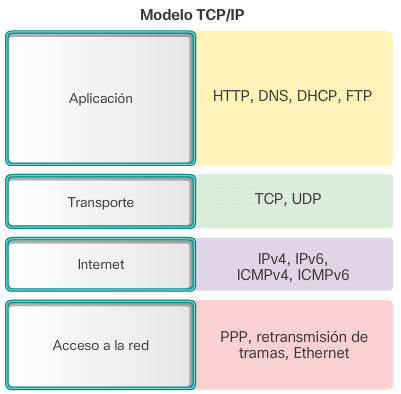
\includegraphics[width=0.8\textwidth]{./Figures/http.png}
	\caption{Modelo TCP/IP y protocolos utilizados en cada capa.}
	\label{fig:capasHTTP}
\end{figure} 

\pagebreak
\section{Componentes de hardware utilizados}

En esta sección se describen los componentes de hardware utilizados, entre los que se incluyen el módulo ESP32, el RFID MRFC-522, el MOSFET IRF520N y la cerradura electrónica.

\subsection{Módulo ESP32}

ESP32 es una familia de chips SoC (System on a Chip) de bajo costo y consumo de energía, con tecnología Wi-Fi y Bluetooth integrada. El mismo emplea un microprocesador Tensilica Xtensa LX6 en las variantes de simple y doble núcleo. Fue creado y desarrollado por Espressif Systems y es fabricado por TSMC utilizando un proceso de 40 nm. Es un sucesor de otro SoC, el ESP8266. ESP32 incluye interruptores de antena, amplificadores de potencia, amplificadores de receptor de bajo ruido, filtros, y módulos de administración de energía. El chip también admite la actualización segura (encriptada) por aire (OTA), para que los desarrolladores puedan actualizar continuamente sus productos, incluso después de su lanzamiento \citep{WEBSITE:esp21wroom}. 

El chip incluye un conjunto de periféricos que son detallados a continuación:
\begin{itemize}
\item 18 canales de convertidor analógico a digital (ADC).
\item 25 pines GPIO, 21 de entrada/salida y 4 de entrada. 10 ellos de pulsación capacitiva.
\item 3 interfaces UART.
\item 3 interfaces SPI.
\item 2 interfaces I2C.
\item 16 canales de salida PWM.
\item 2 convertidores de digital a analógico (DAC).
\item 2 interfaces I2S.
\end{itemize}


En la figura \ref{fig:esp32} puede verse la configuración de pines del ESP32 WROOM32 \citep{WEBSITE:pinesESP32}.

\begin{figure}[ht]
	\centering
	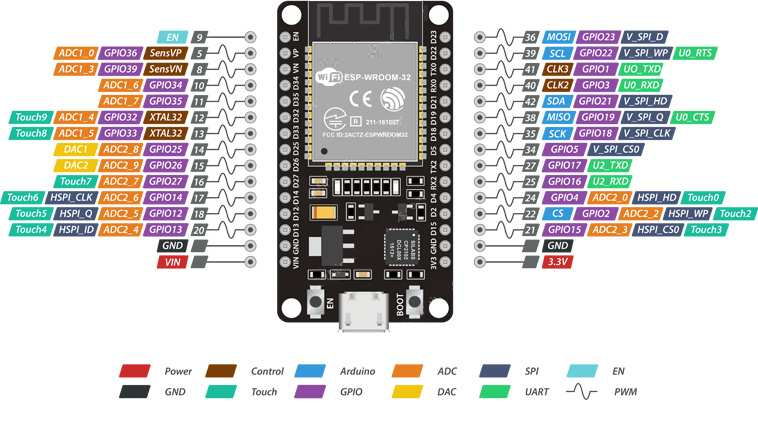
\includegraphics[width=1\textwidth]{./Figures/esp32.png}
	\caption{Pines del ESP32 WROOM32.}
	\label{fig:esp32}
\end{figure} 

\subsection{Módulo RFID MRFC-522}

El módulo RFID MRFC-522 está basado en el circuito integrado MFRC522 de la empresa NXP. Se trata de una de las opciones más económicas y fáciles de usar para la lectura y escritura de tarjetas RFID. El mismo incorpora comunicación a través del bus SPI, bus I2C y UART, por lo que es sencillo de conectar con el ESP32. Opera en la frecuencia de 13.5 6Mhz y tiene una distancia de lectura máxima de 5 cm, mientras que la tensión de alimentación es de 3.3 V. El módulo administra tarjetas o llaveros ``MIFARE Classic 1K''. Este tipo de tarjetas son, esencialmente, un sistema de almacenamiento donde la memoria está dividida en bloques y cuenta con mecanismos simples para el acceso y guardado de la información. Por otro lado soportan más de cien mil ciclos de escritura manteniendo la memoria durante al menos diez años sin recibir alimentación. Debido a esta capacidad, podemos utilizar el módulo para escribir los valores que necesitemos en las tarjetas y leerlos a posteriori. 

\subsubsection{Conexión con ESP32}

En la figura \ref{fig:mrf522} se muestra el modo en el que se conecta el módulo con el ESP32 \citep{WEBSITE:MRF522}. Una vez realizada la conexión puede utilizarse Arduino IDE para el desarrollo de la comunicación entre ambos, valiéndose de las librerías ``MFRC522'' y ``SPI''.

\begin{figure}[ht]
	\centering
	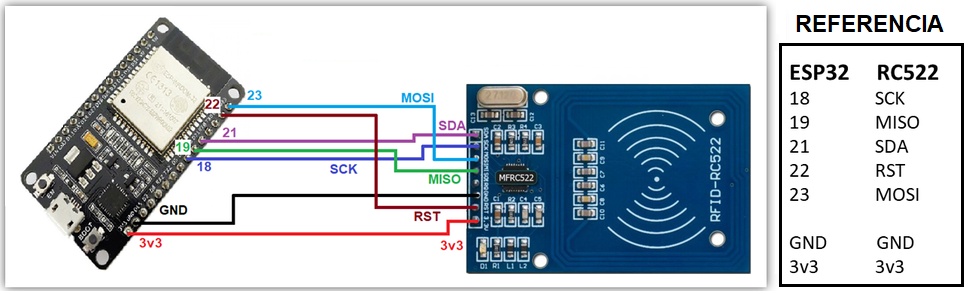
\includegraphics[width=1\textwidth]{./Figures/mrf522.png}
	\caption{Conexión ente módulo MRFC-522 y ESP32.}
	\label{fig:mrf522}
\end{figure} 


\subsection{Módulo MOSFET IRF520N}

El IRF520N es un modelo muy común de transistor MOSFET que se emplea para alimentar cargas a tensión e intensidad superiores a las que podemos proporcionar con las salidas del ESP32 o Arduino. La mayor ventaja del IRF520N es que existen placas comerciales que simplifican significativamente su montaje. Estas placas incluyen resistencias integradas, pines para conectar a Arduino o ESP32 y pines de conexión para conectar la carga \citep{WEBSITE:mosfet}. Al alimentar el módulo con una tensión de 5 V, el IRF520N proporciona a la salida un máximo de 24 V y 4 A. Cabe aclarar que los modelos de ESP32 de 3.3 V no pueden emplear un IRF520N sin pre-amplificación.

Debido a que tiene un excelente desempeño podemos utilizarlo para controlar directamente motores DC con alta demanda de corriente, celdas peltier, tiras de LED o LEDs de alta potencia para reflectores o iluminación, matrices LED, etc. Para utilizar el módulo a toda su capacidad se recomienda agregar un disipador de calor adecuado. En la figura \ref{fig:mosfet} se muestra el módulo MOSFET IRF520 junto a su diagrama de conexión \citep{WEBSITE:mosfetesquemna}.

\begin{figure}[ht]
	\centering
	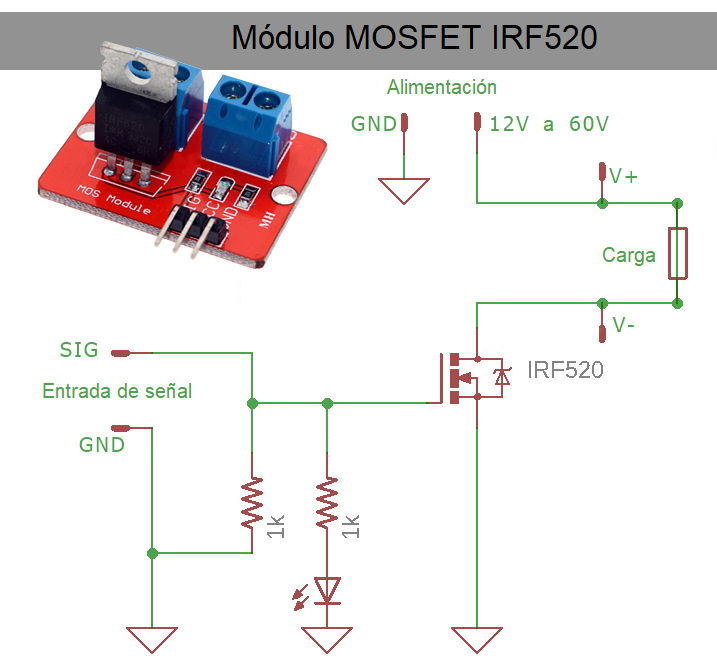
\includegraphics[width=1\textwidth]{./Figures/mosfet.png}
	\caption{módulo MOSFET IRF520 junto a su diagrama de conexión.}
	\label{fig:mosfet}
\end{figure} 


\subsection{Cerradura electrónica}

La cerradura electrónica es un elemento físico que suministra protección de acceso a un bien personal o lugar. No es más que una evolución de la cerradura mecánica tradicional. La principal diferencia radica en que su mecanismo ya no es mecánico, sino electrónico (se hace accionar un electroimán de apertura). Esto quiere decir que no hace falta una llave que la accione, con la ventaja de brindar un acceso controlado y de alta seguridad.

\pagebreak
Actualmente existen dos modos de operación de una cerradura ante un corte eléctrico que son \citep{WEBSITE:trabajoCerradura}:

\begin{itemize}
\item fail secure (si falla, estoy asegurado): cuando no hay suministro eléctrico, la cerradura queda trabada. Este modo de operación se utiliza cuando la prioridad es mantener el lugar cerrado y asegurado.
\item fail safe (si falla, estoy a salvo): trabaja de manera contraria al caso anterior. La cerradura se destraba y la puerta queda abierta. Este modo de operación es muy utilizado cuando la prioridad es la vida de las personas.
\end{itemize}

Para este trabajo se utilizó una cerradura electrónica de pestillo a inducción de marca Cygnus pl-820 como se muestra en la figura \ref{fig:cerradura}. La  cerradura opera con un voltaje de entrada de 12 V y una corriente de 650 mA.

\begin{figure}[ht]
	\centering
	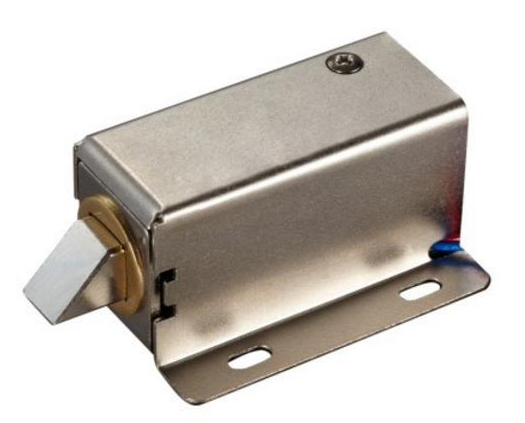
\includegraphics[width=0.6\textwidth]{./Figures/cerradura.png}
	\caption{Cerradura electrónica Cygnus pl-820.}
	\label{fig:cerradura}
\end{figure} 

\pagebreak
\section{Tecnologías de software aplicadas}
 
En esta sección se describen las principales tecnologías de software utilizadas en el trabajo.

\subsection{Node.JS}

Node.js® es un entorno de ejecución multiplataforma, de código abierto, para JavaScript construido con el motor de JavaScript V8 de Chrome \citep{WEBSITE:node}. Está diseñado para crear aplicaciones web escalables y está orientado a eventos asíncronos. Fue creado por Ryan Dahl en 2009.

Node.js funciona con un modelo de ejecución de un único hilo, usando entradas y salidas asíncronas que pueden ejecutarse concurrentemente. Esto requiere que cada solicitud y toda operación que realice entradas y salidas tenga una función de \textit{callback}. Un inconveniente de este enfoque de único hilo de ejecución es que complica el escalamiento de la aplicación, aunque simplifica el modelo de implementación.

Node.js incorpora varios ``módulos básicos'' compilados en el propio binario, como por ejemplo, el módulo de red, que proporciona una capa para programación de red asíncrona y otros módulos fundamentales, como por ejemplo Path, FileSystem, Buffer, Timers y Stream. Es posible a su vez utilizar módulos o librerías desarrolladas por terceros \citep{WEBSITE:nodeWiki}.

En la tabla \ref{tab:nodelibrerias} se muestra el detalle de las librerías utilizadas en Node.JS para nuestro trabajo.

\begin{table}[h]
	\centering
	\caption[Librerías Node.JS]{Librerías utilizadas en Node.JS .}
	\begin{tabular}{p{4cm} p{8.5cm} } 	

		\toprule
		\textbf{Librería} & 
		\textbf{Descripción}
		\\
		\midrule
axios & Cliente HTTP para Javascript. Permite realizar llamadas HTTP POST y GET.\\
bcryptjs & Implementa funciones de hash para guardar los passwords encriptados.\\
express & Framework para generar la aplicación web en Node.JS.\\
cors & Librería para implementar CORS en nuestra solución.\\
jsonwebtoken & Librería para gestionar tokens JWT en nuestra aplicación.\\
mongodb & Librería para conectarnos a la base de datos MongoDB.\\
newman & Librería para ejecutar los test automáticos generados en Postman. \\
Nodemailer & Librearía que permite el envío de emails.\\
pg & Librería para conectarnos a la base de datos PostgreSQL.\\
socket.io & Librería para implementar \textit{WebSockets} en nuestra aplicación.
\\
		\bottomrule
		\hline
	\end{tabular}
	\label{tab:nodelibrerias}
\end{table}

\pagebreak
\subsection{Ionic}

Ionic es un SDK (software developmnet kit) de código abierto para el desarrollo de aplicaciones móviles híbridas creado en 2013 por Max Lynch, Ben Sperry y Adam Bradley de Drifty Co. Mientras la versión original fue implementada sobre AngularJS y Apache Cordova, la versión actual está construida como un conjunto de componentes web. Esto último permite al usuario elegir cualquier framework de interfaz de usuario (Vue, Angular o React) y construirla rápidamente, aprovechando componentes ya armados por terceros o por nosotros mismos con anterioridad. Una de las principales ventajas de Ionic es que nos posibilita desarrollar nuestra aplicación como una \textit{Web App} y luego distribuirla como una \textit{App mobile} en Android o iOS utilizando Cordova o Capacitor, sin necesidad de emplear y aprender las herramientas y lenguajes propios de cada plataforma. Ionic viene por defecto con una serie de componentes, que incluyen cards, grids, tabs y badges \citep{WEBSITE:ionic}.

Dentro de Ionic, utilizamos un conjunto de librerías con componentes ya implementados que permitieron agilizar el desarrollo del sistema. En la tabla \ref{tab:ioniclibrerias} se muestra el listado de librerías y su descripción.

\begin{table}[h]
	\centering
	\caption[Librerías Ionic ]{Librerías utilizadas en Ionic.}
	\begin{tabular}{p{4cm} p{8.5cm} } 	

		\toprule
		\textbf{Librería} & 
		\textbf{Descripción}
		\\
		\midrule
@angular/material & Componentes de interfaz gráfica para Angular. \\
material-design-icons & Librería de íconos. \\
ng2-charts y chart.js & Librerías para armado de gráficos de barra, línea y torta. \\
rxjs & Librería para implementar observables. \\
socket.io-client & Librearía para implementar \textit{WebSockets} del lado del cliente. \\
jwt-decode & Librería para leer tokens JWT y obtener los datos almacenados en los mismos. \\
		\bottomrule
		\hline
	\end{tabular}
	\label{tab:ioniclibrerias}
\end{table}

\pagebreak
\subsection{PostgreSQL}

PostgreSQL es un DBMS (DataBase Management System) de código abierto. Tiene más de 30 años de desarrollo, y cuenta con alta confiabilidad, robustez y performance. Usa y extiende el lenguaje SQL y cumple desde 2001 con las propiedades ACID de las bases de datos relacionales. Los orígenes de PostgreSQL se remontan a 1986 como parte del proyecto POSTGRES en la Universidad de California en Berkeley. Es mantenido por la comunidad PGDG (PostgreSQL Global Development Group).

Además de ser gratuito y de código abierto, PostgreSQL es altamente extensible dado que permite definir sus propios tipos de datos y crear funciones personalizadas. Cuenta con gran cantidad de tipos primitivos, integración de datos, recuperación ante desastres, seguridad y características de internacionalización. Es altamente escalable, tanto por la gran cantidad de datos que puede administrar como por la cantidad de usuarios simultáneos que puede soportar. Hay clústeres activos de PostgreSQL en entornos de producción que administran muchos terabytes de datos y otros sistemas especializados que gestionan petabytes.

\subsection{MongoDB}

MongoDB es un sistema de base de datos NoSQL, orientado a documentos y de código abierto. Su desarrollo comenzó en 2007, y cuando en marzo de 2011 se lanzó la versión 1.4 pasó a ser considerada como una base de datos lista para su uso en producción \citep{WEBSITE:mongo}. MongoDB guarda estructuras de datos BSON (una especificación similar a JSON) con un esquema dinámico, haciendo que la integración de los datos en ciertas aplicaciones sea más fácil y rápida. Está implementado en una gran cantidad de industrias y en grandes empresas como Google, Adobe y Ebay. Está disponible para los sistemas operativos Windows, GNU/Linux, OS X y Solaris. MongoDB es una base de datos distribuida en su núcleo, por lo que la alta disponibilidad, la escalabilidad horizontal y la distribución geográfica están integradas y son fáciles de usar. 

Dentro de las características principales tenemos: 
\begin{itemize}
\item Consultas ad hoc: MongoDB soporta la búsqueda por campos, consultas de rangos y expresiones regulares.
\item Indexación: Cualquier campo en un documento de MongoDB puede ser indexado, al igual que es posible hacer índices secundarios. 
\item Replicación: MongoDB soporta el tipo de replicación primario-secundario. Cuenta con un nodo primario que puede ejecutar comandos de lectura y escritura y varios nodos secundarios que sólo se pueden usar para lectura o para copia de seguridad.
\item Balanceo de carga: MongoDB puede escalar de forma horizontal usando el concepto de \textit{shards}. 
\item Agregación: MongoDB proporciona un framework de agregación que permite realizar operaciones similares al ``GROUP BY'' de SQL.
\item Ejecución de JavaScript del lado del servidor: tiene la capacidad de realizar consultas utilizando JavaScript, haciendo que estas sean enviadas directamente a la base de datos para ser ejecutadas.
\end{itemize}

De acuerdo al ranking de DB-engines \citep{WEBSITE:dbengine}, MongoDB es la base de datos no relacional más utilizada en el mundo. En la figura \ref{fig:mongodb} se muestra el ranking de DB-engines correspondiente a marzo 2021.

\begin{figure}[ht]
	\centering
	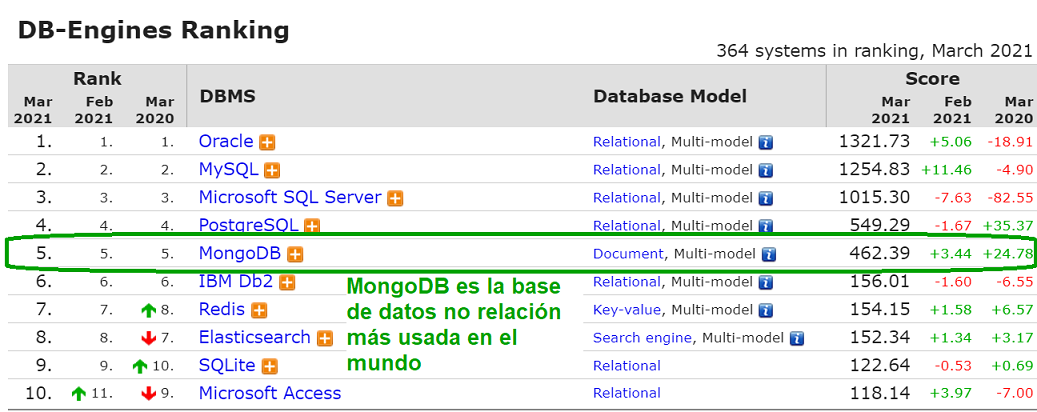
\includegraphics[width=1\textwidth]{./Figures/mongodb.png}
	\caption{Ranking de DB-engines correspondiente a marzo 2021.}
	\label{fig:mongodb}
\end{figure} 

\subsection{Docker}

Docker es una plataforma de código abierto que automatiza el despliegue de aplicaciones dentro de contenedores de software. La misma  permite separar las aplicaciones de la infraestructura, lo cual ayuda a desplegar software rápidamente. Para esto se vale del concepto de contenedores, que son unidades que empaquetan una aplicación junto a sus dependencias. Gracias a esto, el contenedor se puede desplegar como una unidad aislada sin depender de otros componentes, mejorando la seguridad debido a su aislamiento. Es importante mencionar también que estos contenedores son más ligeros que las máquinas virtuales tradicionales. Tales máquinas ejecutan un sistema operativo completo y tienen un conjunto de recursos reservados que solo ellas pueden utilizar como CPU, RAM y disco. En cambio, los contenedores no albergan un sistema operativo completo, sino que todos los que se ejecuten en un mismo equipo comparten los recursos de la infraestructura sobre la que corren. Docker cuenta con una capa de software que gestiona los contenedores, su ejecución y sus recursos y se conoce como ``Docker Engine''.

En la figura \ref{fig:dockerVMs} se muestra las diferencias entre la infraestructura de Docker y las máquinas virtuales.

\begin{figure}[ht]
	\centering
	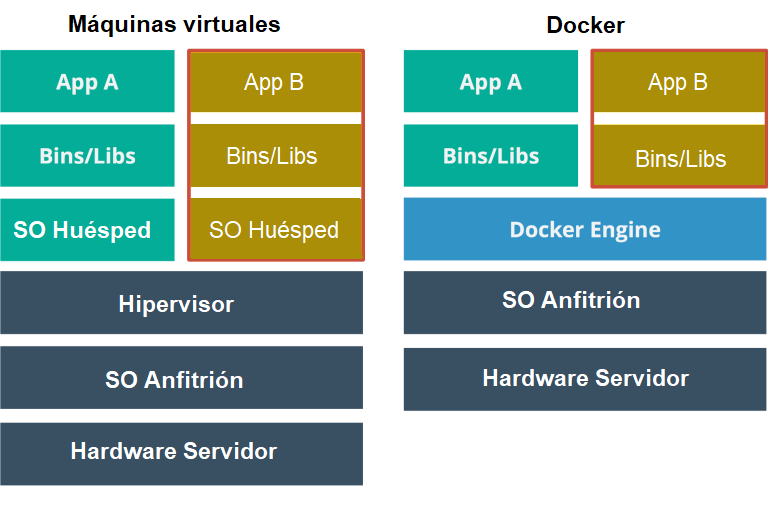
\includegraphics[width=1\textwidth]{./Figures/dockerVMs.png}
	\caption{Diferencia entre la infraestructura de Docker y las máquinas virtuales.}
	\label{fig:dockerVMs}
\end{figure} 

Docker funciona con el concepto de imágenes. Las imágenes son entidades inmutables que actúan como plantillas para la generación de los contenedores. Si bien contienen la aplicación o código a ejecutar, son estáticas. Los contenedores son la ejecución de una imagen particular en un equipo. Puede hacerse una analogía con el concepto de clases y objetos: la clase sería la imagen docker, que tiene el código a ejecutar; mientras que el objeto sería el contenedor en sí, que está en ejecución en un determinado momento y sobre un equipo particular \citep{WEBSITE:dockerredes}.

Cuando tenemos muchos contenedores podemos utilizar un orquestador como Kubernetes, que permite gestionar su alta, reinicio y apagado. También administrar de forma dinámica la cantidad de contenedores de cada tipo, lo que habilita la replicación horizontal. Otra opción más simple, cuando la cantidad de contenedores es baja y no necesitamos gestionar replicación, es utilizar la herramienta docker-compose. Ésta permite, mediante un archivo de configuración, definir los contenedores a utilizar, su configuración, imagen base y dar de alta los mismos automáticamente, a través de una única orden.

\pagebreak
\subsection{Postman}

Postman es un software que está compuesto por diferentes herramientas y utilidades que permiten a los desarrolladores testear las API y lograr una gestión completa de las mismas \citep{WEBSITE:postman1}. El mismo surgió originariamente como una extensión para el navegador Google Chrome y hoy dispone de aplicaciones nativas para MAC, Windows y Linux

Dentro de las características de Postman tenemos \citep{WEBSITE:postman2}: 
\begin{itemize}
\item Crear peticiones: permite generar y enviar peticiones HTTP a servicios REST mediante una interfaz gráfica. Estas peticiones pueden ser guardadas y reproducidas a posteriori.
\item Definir colecciones: posibilita agrupar las APIs en colecciones y establecer el modelo de autenticación de las mismas, de modo que antes de cada test se asegure que el mismo cuenta con las credenciales requeridas. De igual manera, es posible precisar variables que pueden ser usadas por todos los tests de la colección.
\item Gestionar la documentación: permite generar documentación basada en las APIs y colecciones que hemos creado en la herramienta y publicarla.
\item Entorno colaborativo: posibilita compartir las APIs entre equipos de trabajo. Para ello se apoya en una herramienta colaborativa en la nube.
\item Generar código de invocación, dada una API, es capaz de generar el código de invocación para diferentes lenguajes de programación: C, C\#, Go, Java, JavaScript, NodeJS, Objective-C, PHP, Python, Ruby, Shell, Swift, etc.
\item Establecer variables: permite crear variables locales y globales que posteriormente podemos utilizar dentro de nuestras invocaciones o pruebas.
\item Gestión del ciclo de vida de la API: permite gestionar el ciclo de vida de la API, desde su definición, desarrollo, monitoreo y hasta su mantenimiento.
\end{itemize}

\section{Software de control de versiones}

Los sistemas de control de versiones son herramientas de software que ayudan a un equipo de desarrollo a gestionar los cambios en el código fuente a lo largo del tiempo. El software de control de versiones realiza un seguimiento de todas las modificaciones en dicho código. Si se comete un error, los desarrolladores pueden volver a versiones anteriores y comparar el mismo con la versión actual para resolver el error rápidamente. Al mismo tiempo se tiene un log de los cambios realizados y del responsable de dichos cambios. Otra de las ventajas que brinda es que cada integrante puede trabajar en su entorno local y luego centralizar el código completo en un repositorio único compartido por todo el equipo. Esto último permite que diferentes grupos de trabajo mantengan la eficacia y la agilidad a medida que escalan al incluir más desarrolladores.

Dentro de los sistemas de control de versiones uno de los más populares es Git. Git es un proyecto de código abierto maduro y con un mantenimiento activo que desarrolló originalmente Linus Torvalds, en 2005. Es un ejemplo de DVCS (sistema de control de versiones distribuido, por sus siglas en inglés). En lugar de tener un único espacio para todo el historial de versiones del software, como sucede de manera habitual en los sistemas de control de versiones de antaño (CVS o Subversion), en Git, la copia de trabajo del código de cada desarrollador es también un repositorio que puede albergar el historial completo de todos los cambios. Además de contar con una arquitectura distribuida, Git se ha diseñado teniendo en cuenta el rendimiento, la seguridad y la flexibilidad.

\subsection{Gitflow}

Gitflow es un conjunto de extensiones para Git, basado en el modelo de ramificaciones de Vincent Driessen, que facilita el trabajo con los repositorios. Básicamente, Gitflow agrega comandos de alto nivel que, por detrás, usan los comandos tradicionales de Git. De este modo se automatizan convenciones y se simplifica el flujo de trabajo al asignar funciones específicas a las diferentes ramas y definir cómo y cuándo deben interactuar.

Gitflow cuenta con las siguientes ramas \footnote{Para ver detalladamente el proceso de instalación y los comandos utilizados en Gitflow remitirse a \citep{WEBSITE:GitflowDetalle}.}: 

\begin{itemize}
\item Rama master y develop: la rama master tiene el historial de versiones productivas generadas, mientras que develop sirve como rama para integrar las funcionalidades o \textit{features} de la aplicación. 
\item Rama feature: para cada funcionalidad a desarrollar, se genera una rama nueva de feature que una vez completa se une con la rama develop.
\item Rama reléase: una vez que el desarrollo tiene varias funcionalidades listas y probadas se crea una rama de reléase desde la rama de develop. En esta rama solo se incluyen las soluciones de errores, la generación de documentación y otras tareas orientadas a la implementación. Una vez que esta todo listo se une con la rama master y se etiqueta la unión con un número de versión. Además, se une con la rama de develop para transferir los ajustes realizados. 
\item Rama hotfix: se utiliza para hacer correcciones sobre la rama master. Una vez hechos los ajustes necesarios se une tanto a la master, asignándole un número de versión nuevo, como a la develop para transferir los cambios hechos.
\end{itemize}

En la figura \ref{fig:gitflow} se muestran las diferentes ramas de Gitflow.
 
\begin{figure}[ht]
	\centering
	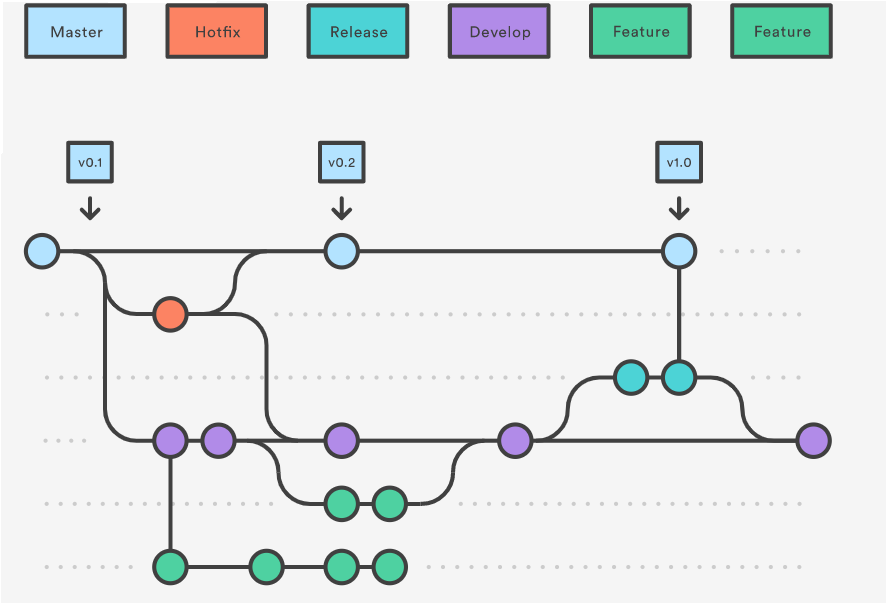
\includegraphics[width=1\textwidth]{./Figures/gitflow.png}
	\caption{Conjunto de ramas de Gitflow}
	\label{fig:gitflow}
\end{figure}  

\pagebreak
\section{Requerimientos}\label{sec:Requerimientos}
 
En esta sección se especifican los requerimientos del proyecto, entre los que se incluyen los funcionales, no funcionales, de documentación y de validación.
 
\subsection{Requerimientos funcionales}
\begin{enumerate}[label=1.\arabic*]
\item El sistema debe permitir el sensado de datos de distintas fuentes y procesos de planta.
\item El sistema deberá generar alertas a usuarios finales ante problemas detectados del sensado o situaciones límites/problemas potenciales.
\item El sistema deberá generar tareas de corrección y prevención con un circuito de estados que permita trazar el origen del problema y la solución asociada.
\item El sistema debe permitir hacer un seguimiento de la cantidad de alarmas diarias y mensuales generadas.
\item El sistema debe permitir hacer un seguimiento de la cantidad de tareas diarias y mensuales generadas A su vez, se deberá poder ver la cantidad de tareas cerradas, en curso y su antigüedad en días.
\item El sistema debe permitir gestionar usuarios para el acceso y utilización del sistema. La gestión de usuarios incluye dar de alta nuevos usuarios y gestionar la recuperación y cambio de clave de los mismos.
\end{enumerate}
\subsection{Requerimientos no funcionales}
\begin{enumerate}[label=2.\arabic*]
\item El sistema deberá ser escalable, de forma de poder agregar a futuro más módulos actuadores y de sensado para los procesos de planta.
\item El sistema deberá ser recuperable ante problemas de hardware o software, de forma de asegurar la disponibilidad y no corrupción de la información, cumpliendo con la política de resguardo de datos de la empresa.
\item El sistema deberá poder operarse aún ante cortes puntuales de energía en algunas áreas. Para ello se deberá contar con una política de suministro alternativo de energía para los servidores donde se ejecute el software. 
\end{enumerate}
\subsection{Requerimientos de documentación}
\begin{enumerate}[label=3.\arabic*]
\item Se debe generar una Memoria Técnica con la documentación de ingeniería detallada.
\item Se debe generar un documento de casos de prueba.
\item Se debe generar un documento de la infraestructura del sistema y de la configuración por ambiente y pasaje entre ambientes.
\item Se deberá generar la documentación del sistema y del proyecto en el sistema de aprobación y documentación TPA de la empresa.
\end{enumerate}
\subsection{Requerimientos de validación}
\begin{enumerate}[label=4.\arabic*]
\item Se deberá tener una matriz de trazabilidad entre los casos de uso y los casos de prueba, validando el cumplimiento de cada uno y con la aprobación final del auspiciante.
\end{enumerate}

